% Options for packages loaded elsewhere
\PassOptionsToPackage{unicode}{hyperref}
\PassOptionsToPackage{hyphens}{url}
\PassOptionsToPackage{dvipsnames,svgnames*,x11names*}{xcolor}
%
\documentclass[
]{article}
\usepackage{amsmath,amssymb}
\usepackage{lmodern}
\usepackage{ifxetex,ifluatex}
\ifnum 0\ifxetex 1\fi\ifluatex 1\fi=0 % if pdftex
  \usepackage[T1]{fontenc}
  \usepackage[utf8]{inputenc}
  \usepackage{textcomp} % provide euro and other symbols
\else % if luatex or xetex
  \usepackage{unicode-math}
  \defaultfontfeatures{Scale=MatchLowercase}
  \defaultfontfeatures[\rmfamily]{Ligatures=TeX,Scale=1}
\fi
% Use upquote if available, for straight quotes in verbatim environments
\IfFileExists{upquote.sty}{\usepackage{upquote}}{}
\IfFileExists{microtype.sty}{% use microtype if available
  \usepackage[]{microtype}
  \UseMicrotypeSet[protrusion]{basicmath} % disable protrusion for tt fonts
}{}
\makeatletter
\@ifundefined{KOMAClassName}{% if non-KOMA class
  \IfFileExists{parskip.sty}{%
    \usepackage{parskip}
  }{% else
    \setlength{\parindent}{0pt}
    \setlength{\parskip}{6pt plus 2pt minus 1pt}}
}{% if KOMA class
  \KOMAoptions{parskip=half}}
\makeatother
\usepackage{xcolor}
\IfFileExists{xurl.sty}{\usepackage{xurl}}{} % add URL line breaks if available
\IfFileExists{bookmark.sty}{\usepackage{bookmark}}{\usepackage{hyperref}}
\hypersetup{
  pdftitle={BDA - Assignment X},
  pdfauthor={Anonymous},
  colorlinks=true,
  linkcolor=Maroon,
  filecolor=Maroon,
  citecolor=Blue,
  urlcolor=blue,
  pdfcreator={LaTeX via pandoc}}
\urlstyle{same} % disable monospaced font for URLs
\usepackage[margin=1in]{geometry}
\usepackage{color}
\usepackage{fancyvrb}
\newcommand{\VerbBar}{|}
\newcommand{\VERB}{\Verb[commandchars=\\\{\}]}
\DefineVerbatimEnvironment{Highlighting}{Verbatim}{commandchars=\\\{\}}
% Add ',fontsize=\small' for more characters per line
\usepackage{framed}
\definecolor{shadecolor}{RGB}{248,248,248}
\newenvironment{Shaded}{\begin{snugshade}}{\end{snugshade}}
\newcommand{\AlertTok}[1]{\textcolor[rgb]{0.94,0.16,0.16}{#1}}
\newcommand{\AnnotationTok}[1]{\textcolor[rgb]{0.56,0.35,0.01}{\textbf{\textit{#1}}}}
\newcommand{\AttributeTok}[1]{\textcolor[rgb]{0.77,0.63,0.00}{#1}}
\newcommand{\BaseNTok}[1]{\textcolor[rgb]{0.00,0.00,0.81}{#1}}
\newcommand{\BuiltInTok}[1]{#1}
\newcommand{\CharTok}[1]{\textcolor[rgb]{0.31,0.60,0.02}{#1}}
\newcommand{\CommentTok}[1]{\textcolor[rgb]{0.56,0.35,0.01}{\textit{#1}}}
\newcommand{\CommentVarTok}[1]{\textcolor[rgb]{0.56,0.35,0.01}{\textbf{\textit{#1}}}}
\newcommand{\ConstantTok}[1]{\textcolor[rgb]{0.00,0.00,0.00}{#1}}
\newcommand{\ControlFlowTok}[1]{\textcolor[rgb]{0.13,0.29,0.53}{\textbf{#1}}}
\newcommand{\DataTypeTok}[1]{\textcolor[rgb]{0.13,0.29,0.53}{#1}}
\newcommand{\DecValTok}[1]{\textcolor[rgb]{0.00,0.00,0.81}{#1}}
\newcommand{\DocumentationTok}[1]{\textcolor[rgb]{0.56,0.35,0.01}{\textbf{\textit{#1}}}}
\newcommand{\ErrorTok}[1]{\textcolor[rgb]{0.64,0.00,0.00}{\textbf{#1}}}
\newcommand{\ExtensionTok}[1]{#1}
\newcommand{\FloatTok}[1]{\textcolor[rgb]{0.00,0.00,0.81}{#1}}
\newcommand{\FunctionTok}[1]{\textcolor[rgb]{0.00,0.00,0.00}{#1}}
\newcommand{\ImportTok}[1]{#1}
\newcommand{\InformationTok}[1]{\textcolor[rgb]{0.56,0.35,0.01}{\textbf{\textit{#1}}}}
\newcommand{\KeywordTok}[1]{\textcolor[rgb]{0.13,0.29,0.53}{\textbf{#1}}}
\newcommand{\NormalTok}[1]{#1}
\newcommand{\OperatorTok}[1]{\textcolor[rgb]{0.81,0.36,0.00}{\textbf{#1}}}
\newcommand{\OtherTok}[1]{\textcolor[rgb]{0.56,0.35,0.01}{#1}}
\newcommand{\PreprocessorTok}[1]{\textcolor[rgb]{0.56,0.35,0.01}{\textit{#1}}}
\newcommand{\RegionMarkerTok}[1]{#1}
\newcommand{\SpecialCharTok}[1]{\textcolor[rgb]{0.00,0.00,0.00}{#1}}
\newcommand{\SpecialStringTok}[1]{\textcolor[rgb]{0.31,0.60,0.02}{#1}}
\newcommand{\StringTok}[1]{\textcolor[rgb]{0.31,0.60,0.02}{#1}}
\newcommand{\VariableTok}[1]{\textcolor[rgb]{0.00,0.00,0.00}{#1}}
\newcommand{\VerbatimStringTok}[1]{\textcolor[rgb]{0.31,0.60,0.02}{#1}}
\newcommand{\WarningTok}[1]{\textcolor[rgb]{0.56,0.35,0.01}{\textbf{\textit{#1}}}}
\usepackage{graphicx}
\makeatletter
\def\maxwidth{\ifdim\Gin@nat@width>\linewidth\linewidth\else\Gin@nat@width\fi}
\def\maxheight{\ifdim\Gin@nat@height>\textheight\textheight\else\Gin@nat@height\fi}
\makeatother
% Scale images if necessary, so that they will not overflow the page
% margins by default, and it is still possible to overwrite the defaults
% using explicit options in \includegraphics[width, height, ...]{}
\setkeys{Gin}{width=\maxwidth,height=\maxheight,keepaspectratio}
% Set default figure placement to htbp
\makeatletter
\def\fps@figure{htbp}
\makeatother
\setlength{\emergencystretch}{3em} % prevent overfull lines
\providecommand{\tightlist}{%
  \setlength{\itemsep}{0pt}\setlength{\parskip}{0pt}}
\setcounter{secnumdepth}{-\maxdimen} % remove section numbering
\ifluatex
  \usepackage{selnolig}  % disable illegal ligatures
\fi

\title{BDA - Assignment X}
\author{Anonymous}
\date{}

\begin{document}
\maketitle

{
\hypersetup{linkcolor=}
\setcounter{tocdepth}{1}
\tableofcontents
}
\hypertarget{introduction}{%
\section{Introduction}\label{introduction}}

This is a template with format instructions for Assignments in the
Bayesian Data Analysis course at Aalto University. R markdown is a
convenient way of writing exercise reports by combining text and R code
using markdown syntax. To create your assignment, remove the formatting
instructions and use this file as a template. Keep the header (the first
lines of this file between two lines of ---) as it sets the author name
to be anonymous, and you can set the title to match the assignment
number.

R markdown makes it easy to make a structured document with section and
subsection titles, textual explanations, equations, code and figures in
logical order. When you make changes to the code and re-run the notebook
or ``knit'' (render) it to PDF, the relevant code is re-run and the
figures and results are updated without need to copy and past (which is
probe to errors).

To edit R Markdown you can use any editor, but RStudio's visual R
markdown editor is probably easiest, as you immediately see how it looks
and can choose formatting (e.g.~section headings, bolding, lists,
figures, etc.) from the toolbar.

More information on how to use markdown, see
\url{https://github.com/adam-p/markdown-here/wiki/Markdown-Cheatsheet}
and more information on R markdown can be found at
\url{https://www.rstudio.com/wp-content/uploads/2015/02/rmarkdown-cheatsheet.pdf}.

Also, \emph{R Markdown: The Definite Guide}, an extensive book on R
Markdown can be found at \url{https://bookdown.org/yihui/rmarkdown/}.

\textbf{Note} The report should be anonymous and submitted to
\url{peergrade.io} as \texttt{assignmentX.pdf}. If you have problem with
creating a PDF file directly from R markdown, start by creating an HTML
file and the just print the HTML to a PDF. You may also use other
software to create the report pdf, but follow the general instructions
in this file (see the
\href{https://github.com/avehtari/BDA_course_Aalto/blob/master/templates/assignment_template.pdf}{pdf
version this file}).

\hypertarget{loaded-packages}{%
\section{Loaded packages}\label{loaded-packages}}

Below are examples of how to load packages that are used in the
assignment. After installing the \texttt{aaltobda} package, you need to
also load it in the beginning of every notebook where you want to use it
with \texttt{library()} function:

\begin{Shaded}
\begin{Highlighting}[]
\CommentTok{\# To install aaltobda, see the General information in the assignment.}
\FunctionTok{library}\NormalTok{(aaltobda)}
\end{Highlighting}
\end{Shaded}

\hypertarget{including-source-code}{%
\section{Including source code}\label{including-source-code}}

In general, all code needed to produce the essential parts needs to be
included, so that it is possible to see, for peer reviewers (and TAs),
where errors may have happened.

You can always look at the open rubrics to see how and what is asked for
in each exercise.

Try to avoid printing an excessive amount of code and think about what
is essential for showing how did you get the result.

Write clear code. The code is also part of your report and clarity of
the report affects your score. If the code is not self-explanatory, add
comments. In a notebook, you can interleave explaining text and code.

If in doubt additional source code can be included in an appendix.

\hypertarget{format-instructions}{%
\section{Format instructions}\label{format-instructions}}

All exercises in the assignment should start with a header fully
specifying that it is exercise X, as (in rmd use \#):

\hypertarget{exercise-1}{%
\section{Exercise 1)}\label{exercise-1}}

Subtasks in each assignments should be numbered and use header (in rmd
use \#\#).

\hypertarget{a}{%
\subsection{a)}\label{a}}

For each subtask include necessary textual explanation, equations, code
and figures so that the answer to the question flows naturally. You can
think what kind of report would you like to review, and what kind of
information would make it easier where there is error (if there are
errors).

\hypertarget{code}{%
\section{Code}\label{code}}

We can easily add R code as chunks in the following way:

\begin{Shaded}
\begin{Highlighting}[]
\DecValTok{5} \SpecialCharTok{+} \DecValTok{5}
\end{Highlighting}
\end{Shaded}

\begin{verbatim}
## [1] 10
\end{verbatim}

This R code is evaluated when running the notebook or when rendering to
PDF.

If you want to show and run the code, but the output is very long or
messy and you prefer to hide the output from the rendered report you can
use option results=`hide'. This is useful especially later as Stan may
output many lines.

\begin{Shaded}
\begin{Highlighting}[]
\DecValTok{5} \SpecialCharTok{+} \DecValTok{5}
\end{Highlighting}
\end{Shaded}

If you want to use some code in the notebook, but think it's not helpful
for the reviewers you can exclude it from the generated PDF with option
\texttt{include=FALSE}. You will see the next block in rmd, but not in
the generated PDF.

\hypertarget{plots}{%
\section{Plots}\label{plots}}

Include plots, where we can specify the width and height of the figure.

\begin{Shaded}
\begin{Highlighting}[]
\FunctionTok{data}\NormalTok{(}\StringTok{"drowning"}\NormalTok{) }\CommentTok{\# Access the data in aaltobda package}
\FunctionTok{plot}\NormalTok{(drowning}\SpecialCharTok{$}\NormalTok{year, drowning}\SpecialCharTok{$}\NormalTok{drownings)}
\end{Highlighting}
\end{Shaded}

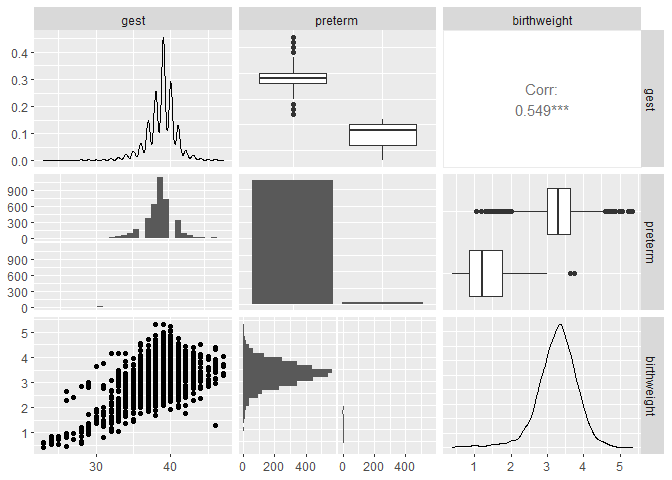
\includegraphics{00_template_files/figure-latex/unnamed-chunk-5-1.pdf}

Or using qplot from ggplot2 package

\begin{Shaded}
\begin{Highlighting}[]
\FunctionTok{library}\NormalTok{(ggplot2)}
\end{Highlighting}
\end{Shaded}

\begin{verbatim}
## Warning: package 'ggplot2' was built under R version 4.0.5
\end{verbatim}

\begin{Shaded}
\begin{Highlighting}[]
\FunctionTok{qplot}\NormalTok{(drowning}\SpecialCharTok{$}\NormalTok{year, drowning}\SpecialCharTok{$}\NormalTok{drownings)}\SpecialCharTok{+}
  \FunctionTok{labs}\NormalTok{(}\AttributeTok{x=}\StringTok{"Year"}\NormalTok{, }\AttributeTok{y=}\StringTok{"Drownings"}\NormalTok{)}
\end{Highlighting}
\end{Shaded}

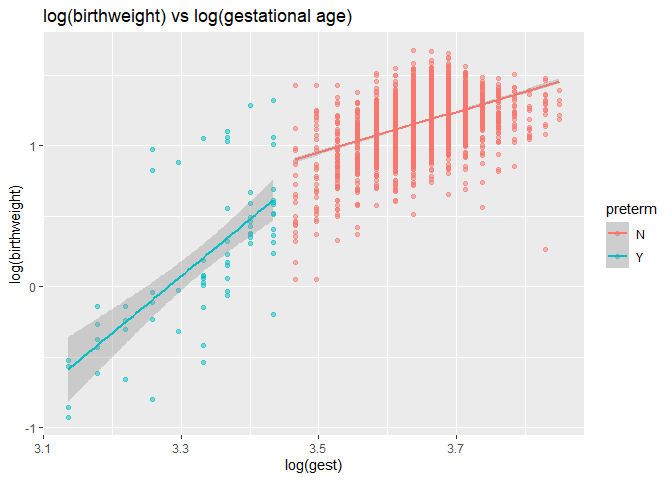
\includegraphics{00_template_files/figure-latex/unnamed-chunk-6-1.pdf}

Or using ggplot from ggplot2 package

\begin{Shaded}
\begin{Highlighting}[]
\FunctionTok{ggplot}\NormalTok{(}\AttributeTok{data=}\NormalTok{drowning, }\FunctionTok{aes}\NormalTok{(}\AttributeTok{x=}\NormalTok{year, }\AttributeTok{y=}\NormalTok{drownings)) }\SpecialCharTok{+} 
  \FunctionTok{geom\_point}\NormalTok{() }\SpecialCharTok{+}
  \FunctionTok{labs}\NormalTok{(}\AttributeTok{x=}\StringTok{\textquotesingle{}Year\textquotesingle{}}\NormalTok{, }\AttributeTok{y=}\StringTok{\textquotesingle{}Number of drownings\textquotesingle{}}\NormalTok{)}
\end{Highlighting}
\end{Shaded}

\includegraphics{00_template_files/figure-latex/unnamed-chunk-7-1.pdf}

\hypertarget{images}{%
\section{Images}\label{images}}

You can include an existing image (e.g.~scanned copy of pen and paper
equations)

\begin{figure}
\centering
\includegraphics[width=3.64583in,height=\textheight]{bayes_workflow.jpg}
\caption{Parts of Bayesian workflow}
\end{figure}

or alternatively

\begin{Shaded}
\begin{Highlighting}[]
\CommentTok{\# knitr::include\_graphics("bayesian\_workflow\_illustration.pdf")}
\end{Highlighting}
\end{Shaded}

\hypertarget{equations}{%
\section{Equations}\label{equations}}

You can write equations using LaTeX syntax, or you can include them as
images if, for example, you use Microsoft Equations.

In Markdown, equations can easily be formulated using LaTeX in line as
\(f(k) = {n \choose k} p^{k} (1-p)^{n-k}\). Or use the math environment
as follows:

\[
\begin{array}{ccc}
x_{11} & x_{12} & x_{13}\\
x_{21} & x_{22} & x_{23}.
\end{array}
\]

The above example illustrated also multicolumn `array'. Alternative way
to make multiline equations with alignment is to use `aligned' as
follows; \[
\begin{aligned}
y & \sim \mathrm{normal}(\mu,1) \\
\mu & \sim \mathrm{normal}(0,1).
\end{aligned}
\]

If you are new to LaTeX equations, you could use the
\href{https://www.latex4technics.com/}{latext4technics} equation editor
to create LaTeX equations to include in the report.

More information on using LaTeX in R markdown can be found in 2.5.3 in
\href{https://bookdown.org/yihui/rmarkdown/}{R Markdown: The Definite
Guide}.

A short introduction to equations in LaTeX can be found at
\url{https://www.overleaf.com/learn/latex/Mathematical_expressions}.

\hypertarget{language}{%
\section{Language}\label{language}}

The language used in the course is English. Hence the report needs to be
written in English.

\hypertarget{jupyter-notebook-and-other-report-formats}{%
\section{Jupyter Notebook and other report
formats}\label{jupyter-notebook-and-other-report-formats}}

You are allowed to use any format to produce your report, such as
Jupyter Notebook, as long as you follow the formatting instructions in
this template.

\end{document}
